\documentclass[a4paper,english,11pt]{article}
\usepackage{a4a}

\begin{document}

\title{Stock assessment with the \aFa statistical catch-at-age framework}

\author[1]{Ernesto Jardim}
\author[1,2,3]{Colin Millar}
\affil[1]{European Commission, Joint Research Centre, Sustainable resources directorate, Water and Marine Resources unit, 21027 Ispra (VA), Italy}
\affil[3]{International Council for the Exploration of the Sea (ICES), H. C. Andersens Boulevard 44-46, 1553 Copenhagen V, Denmark}
\affil[*]{Corresponding author \href{mailto:ernesto.jardim@ec.europa.eu}{ernesto.jardim@ec.europa.eu}}


\maketitle

\begin{abstract}
This chapter presents the statistical catch-at-age stock assessment model developed as part of the Assessment For All (\aFa) initiative of the European Commission Joint Research Centre. The stock assessment model framework is a non-linear catch-at-age model implemented in \href{http://www.r-project.org/}{\R}, \href{http://www.flr-project.org/}{\FLR} and \href{http://www.admb-project.org/}{\ADMB}, that can be applied rapidly to a wide range of situations with low parametrization requirements. The model structure is defined by submodels, which are the different parts that require structural assumptions. There are 5 submodels in operation: F-at-age, abundance indices catchability-at-age, recruitment, observation variance of catch-at-age and abundance indices-at-age, and population's age structurein the first year. All submodels use the same type of specification process, the \R formula interface, wich gives lot's of flexibility to explore models and combination of submodels.
\end{abstract}

\newpage
\tableofcontents
\newpage



\section{Before starting}

\subsection{License, documentation and development status}

The software is released under the \href{https://joinup.ec.europa.eu/community/eupl/home}{EUPL 1.1}.

For more information on the \aFa methodologies refer to \href{http://icesjms.oxfordjournals.org/content/early/2014/04/03/icesjms.fsu050.abstract}{Jardim, et.al, 2014}, \href{http://icesjms.oxfordjournals.org/content/early/2014/03/31/icesjms.fsu043.abstract}{Millar, et.al, 2014} and \href{http://journals.plos.org/plosone/article?id=10.1371/journal.pone.0154922}{Scott, et.al, 2016}.

Documentation can be found at \url{http://flr-project.org/FLa4a}. You are welcome to:

\begin{itemize}
	\item Submit suggestions and bug-reports at: \url{https://github.com/flr/FLa4a/issues}
	\item Send a pull request on: \url{https://github.com/flr/FLa4a/}
	\item Compose a friendly e-mail to the maintainer, see `packageDescription('FLa4a')`
\end{itemize}

\subsection{Installing and loading libraries}

To run the \code{FLa4a} methods the reader will need to install the package and its dependencies and load them. Some datasets are distributed with the package and as such need to be loaded too.

\begin{knitrout}
\definecolor{shadecolor}{rgb}{0.949, 0.949, 0.949}\color{fgcolor}\begin{kframe}
\begin{alltt}
\hlcom{# from CRAN}
\hlkwd{install.packages}\hldef{(}\hlkwd{c}\hldef{(}\hlsng{"copula"}\hldef{,} \hlsng{"triangle"}\hldef{,} \hlsng{"coda"}\hldef{,} \hlsng{"grid"}\hldef{,} \hlsng{"gridExtra"}\hldef{,} \hlsng{"latticeExtra"}\hldef{))}
\hlcom{# from FLR}
\hlkwd{install.packages}\hldef{(}\hlkwd{c}\hldef{(}\hlsng{"FLCore"}\hldef{,} \hlsng{"FLa4a"}\hldef{),} \hlkwc{repos} \hldef{=} \hlsng{"http://flr-project.org/R"}\hldef{)}
\end{alltt}
\end{kframe}
\end{knitrout}

\begin{knitrout}
\definecolor{shadecolor}{rgb}{0.949, 0.949, 0.949}\color{fgcolor}\begin{kframe}
\begin{alltt}
\hlcom{# libraries}
\hlkwd{library}\hldef{(devtools)}
\hlkwd{library}\hldef{(FLa4a)}
\hlkwd{library}\hldef{(XML)}
\hlkwd{library}\hldef{(reshape2)}
\hlkwd{library}\hldef{(ggplotFL)}
\hlcom{# datasets}
\hlkwd{data}\hldef{(ple4)}
\hlkwd{data}\hldef{(ple4.indices)}
\hlkwd{data}\hldef{(ple4.index)}
\hlkwd{data}\hldef{(rfLen)}
\end{alltt}
\end{kframe}
\end{knitrout}

\begin{knitrout}
\definecolor{shadecolor}{rgb}{0.949, 0.949, 0.949}\color{fgcolor}\begin{kframe}
\begin{alltt}
\hlkwd{packageVersion}\hldef{(}\hlsng{"FLCore"}\hldef{)}
\end{alltt}
\begin{verbatim}
## [1] '2.6.20.920'
\end{verbatim}
\begin{alltt}
\hlkwd{packageVersion}\hldef{(}\hlsng{"FLa4a"}\hldef{)}
\end{alltt}
\begin{verbatim}
## [1] '1.9.0'
\end{verbatim}
\end{kframe}
\end{knitrout}

\subsection{How to read this document}

The target audience for this document are readers with some experience in R and some background on stock assessment.

The document explains the approach being developed by \aFa for fish stock assessment and scientific advice. It presents a mixture of text and code, where the first explains the concepts behind the methods, while the last shows how these can be run with the software provided. Moreover, having the code allows the reader to copy/paste and replicate the analysis presented here.

The sections and subsections are as independent as possible, so it can be used as a reference document for the \code{FLa4a}. 

\subsection{Notation}

Along this chapter the notation presented in Table~\ref{tab:mathsnotation} will be used. Mathematical descriptions will be kept as simple as possible for readability.

\begin{table}
  \caption{Mathematical notation}
  \label{tab:mathsnotation}

  \begin{center}
    \begin{tabular}{cc}
      \hline
      Symbol & Description \\
      \hline
      \hline
       Variables & \\
       $C$ & catches \\
       $F$ & fishing mortality \\
       $M$ & natural mortality \\
       $R$ & recruitment \\
       $Q$ & vessel or fleet catchability \\
       $w$ & weights \\
       $l$ & likelihood \\
       $I$ & abundance index \\
       $S$ & spawning stock biomass \\
       $CV$ & coefficient of variation \\
       $D$ & residuals or deviances \\
       $N$ & normal distribution \\
       $\beta$ & parameter \\
       $a$ & stock-recruitment parameter \\
       $b$ & stock-recruitment parameter \\
       $\sigma^2$ & variance of catch \\
       $\tau^2$ & variance of index \\
       $\phi^2$ & variance of predicted recruitment \\
       $\upsilon^2$ & variance of residuals \\
       Subscripts & \\
       $a$ & age \\
       $y$ & year \\
       $C$ & catch \\
       $I$ & abundance index \\
       $N$ & normal distribution \\
       $s$ & survey \\
       $SR$ & stock recruitment relationship \\
       Superscripts and accents & \\
       $\hat{}$ & observation \\
       $\tilde{}$ & prediction \\
       $c$ & catches \\
       $s$ & abundance index \\
      \hline
    \end{tabular}
  \end{center}
\end{table}

\section{Introduction}

The \aFa stock assessment framework is based in a non-linear catch-at-age model implemented in \R, \FLR and \ADMB that can be applied rapidly to a wide range of situations with low setup requirements.

The framework is built of submodels which define the different parts of a statistical catch at age model that require structural assumptions. In the \aFa framework these are fishing mortality-at-age, abundance indicies catchability-at-age, recruitment, observation variances of catch-at-age and abundance indices-at-age, and abundance-at-age in the first year of the data series (see section~\ref{sec:math} for details).

Other important processes, like natural mortality, individual growth and reproduction, are treated as fixed(inputs??), as it's common in stock assessment methods. Nevertheless, the \aFa framework provides methods to condition these processes prior to the model fit, and propagate their uncertainty into the assessment process. See chapters XX and section XX.

The submodels formulation uses linear models, which opens the possibility of using the linear modelling tools available in \R. For example, \href{http://cran.r-project.org/web/packages/mgcv/index.html}{\code{mgcv}} gam formulas or factorial design formulas using \code{lm()}.

The 'language' of linear models has been developing within the statistical community for many years, and constitutes an elegant way of defining models without going through the complexity of mathematical representations. This approach makes it also easier to communicate among scientists:
\begin{itemize}
  \item \href{http://rspa.royalsocietypublishing.org/content/283/1393/147.short}{1965 J. A. Nelder}, notation for randomized block design
  \item \href{http://www.jstor.org/stable/info/2346786}{1973 Wilkinson and Rodgers}, symbolic description for factorial designs
  \item \href{http://books.google.com/books?isbn=0412343908}{1990 Hastie and Tibshirani}, introduced notation for smoothers
  \item \href{http://books.google.com/books?isbn=041283040X}{1991 Chambers and Hastie}, further developed for use in S
\end{itemize}

\section{Stock assessment framework maths description}\label{sec:math}

The stock assessment model behind the framework is based in two main equations to link observations to processes, the Baranov's catch equation and abundance indices equation.

Catches in numbers by age and year are defined in terms of the three quantities: natural mortality, fishing mortality and recruitment; using a modified form of the well known Baranov catch equation:

$$C_{ay} = \frac{F_{ay}}{F_{ay}+M_{ay}}\left(1 - e^{-(F_{ay}+M_{ay})}\right) R_{y}e^{-\sum (F_{ay} + M_{ay})} $$

Survey indices by age and year are defined in terms of the same three quantities with the addition of survey catchability:

$$I_{ays} = Q_{ays} R_{y}e^{-\sum (F_{ay} + M_{ay})}$$

Observed catches and observed survey indices are assumed to be log-normally distributed, or equivalently, normally distributed on the log-scale, with specific observation variance:

$$ \log \hat{C}_{ay} \sim \text{Normal} \Big( \log C_{ay}, \sigma^2_{ay}\Big) $$
$$ \log \hat{I}_{ays} \sim \text{Normal} \Big( \log I_{ays}, \tau^2_{ays} \Big) $$

The log-likelihood can now be defined as the sum of the log-likelihood of the observed catches:

$$  \ell_C = \sum_{ay} w^{(c)}_{ay}\ \ell_N \Big( \log C_{ay}, \sigma^2_{ay} ;\ \log \hat{C}_{ay} \Big) $$

and the log-likelihood of the observed survey indices as:

$$  \ell_I = \sum_s \sum_{ay} w^{(s)}_{ays}\ \ell_N \Big( \log I_{ays}, \tau_{ays}^2 ;\ \log \hat{I}_{ays} \Big)$$

giving the total log-likelihood

$$\ell = \ell_C + \ell_I$$

which is defined in terms of the strictly positive quantites, $M_{ay}$, $F_{ay}$, $Q_{ays}$ and $R_{y}$, and the observation variances $\sigma_{ay}$ and $\tau_{ays}$. As such, the log-likelihood is over-parameterised as there are many more parameters than observations. In order to reduce the number of parameters, $M_{ay}$ is assumed known (as is common). 

%====================================================================
%THE FOLLOWING NEEDS REVISION, need to bring in N1 submod
%====================================================================

The remaining parameters are written in terms of a linear combination of covariates $x_{ayk}$, e.g.

$$\log F_{ay} = \sum_k \beta_k x_{ayk}$$

where $k$ is the number of parameters to be estimated and is sufficiently small. Using this tecnique the quantities $\log F$, $\log Q$, $\log \sigma$ and $\log \tau$
%$\log \text{initial\,age\,structure}$ % this is not present in the above
(in bold in the equations above) can be described by a reduced number of parameters. The following section has more discussion on the use of linear models in \aFa.

%====================================================================

The \aFa statistical catch-at-age model can addionally allow for a functional relationship that links predicted recruitment $\tilde{R}$ based on spawning stock biomass and modelled recruitment $R$, to be imposed as a fixed variance random effect. [NEEDS REVISION, sentence not clear]

Options for the relationship are the hard coded models Ricker, Beverton Holt, smooth hockeystick or geometric mean. This is implemented by including a third component in the log-likelihood:

$$\ell_{SR} = \sum_y \ell_N \Big( \log \tilde{R}_y(a, b), \phi_y^2 ;\ \log R_y \Big)$$

giving the total log-likelihood

$$\ell = \ell_C + \ell_I + \ell_{SR}$$

Using the (time varying) Ricker model as an example, predicted recruitment is

$$\tilde{R}_y(a_y,b_y) = a_y S_{y-1} e^{-b_y S_{y-1}}$$

where $S$ is spawning stock biomass derived from the model parameters $F$ and $R$, and the fixed quantites $M$ and mean weights by year and age. It is assumed that $R$ is log-normally distributed, or equivalently, normally distributed on the log-scale about the (log) recruitment predicted by the SR model $\tilde{R}$, with known variance $\phi^2$, i.e.

$$\log R_y \sim \text{Normal} \Big( \log \tilde{R}_y, \phi_y^2 \Big)$$

which leads to the definition of $\ell_{SR}$ given above. In all cases $a$ and $b$ are strictly positive, and with the quantities $F$, $R$, etc. linear models are used to parameterise $\log a$ and/or $\log b$, where relevant.

%====================================================================
%THE FOLLOWING NEEDS REVISION, this is not just the default I guess, 
% it's always present since R predictions will be a mix of S/R and $\gamma$
%====================================================================

By default, recruitment $R$ as apposed to the reruitment predicted from a stock recruitment model $\tilde{R}$, is specified as a linear model with a parameter for each year, i.e.

$$\log R_y = \gamma_y$$

This is to allow modelled recruitment $R_y$ to be shrunk towards the stock recruitment model. However, if it is considered appropriate that recruitment can be determined exactly by a relationship with covariates, it is possible, to instead define $\log R$ in terms of a linear model in the same way as $\log F$, $\log Q$, $\log \sigma$ and $\log \tau$.  %But this is pretty much the same as taking a geometric mean, with a model on log a, and making the variance very small.

%====================================================================
% WE NEED TO ADD SOMETHING ABOUT HOW THE PLUSGROUP IS MODELLED
%====================================================================

%====================================================================

\section{Submodel structure}\label{sec:submod}

The \aFa stock assessment framework allows the user to set up a large number of different models. The mechanics which provide this flexibility are designed around the concept of submodels. Each unknown variable that must be estimated is treated as a linear model, for which the user has to define the model structure using \R formulas, including \href{http://cran.r-project.org/web/packages/mgcv/index.html}{\code{mgcv}} gam formulas. All submodels use the same specification process, the \R formula interface, wich gives lot's of flexibility to explore models and combination of submodels.

There are 5 submodels in operation:
\begin{itemize}
  \item a model for F-at-age ($F_{ay}$),
  \item a (list) of model(s) for abundance indices catchability-at-age ($Q_{ays}$),
  \item a model for recruitment ($R_y$),
  \item a list of models for the observation variance of catch-at-age and abundance indices ($\{\sigma^2_{ay}, \tau^2_{ays}\}$),
  \item a model for the initial age structure $N_{a,y=1}$,
\end{itemize}

When setting the structure of each submodel the user is in fact building the predictive model and its parameters. The optimization process, done through \ADMB, estimates the parameters and their variance-covariance matrix, allowing further analysis to be carried out, like simulation, prediction, diagnostics, etc. All the statistical machinery will be at the user's reach.

\subsection{Submodel building blocks and fundamental R formulas}

The elements available to build submodels formulas are 'age' and 'year', which can be used to build models with different structures. 

In \R's linear modelling language, a constant model is coded as \code{\midtilde 1}, while a slope over time would simply be \code{\midtilde year}, a smoother over time \code{\midtilde s(year, k=10)}, a model with a coefficient for each year (also called dummy variables) would be \code{\midtilde factor(year)}. Transformations of the variables are as usual, e.g. \code{\midtilde sqrt(year)}, etc; while combinations of all the above can be done non-convergence will limit the possibilities. 

Using the $F$ submodel as example the following specifies the models described in the previous paragraph:

\begin{knitrout}
\definecolor{shadecolor}{rgb}{0.949, 0.949, 0.949}\color{fgcolor}\begin{kframe}
\begin{alltt}
\hlcom{# models}
\hldef{m1} \hlkwb{<-} \hlopt{~}\hlnum{1}
\hldef{m2} \hlkwb{<-} \hlopt{~}\hldef{year}
\hldef{m3} \hlkwb{<-} \hlopt{~}\hlkwd{s}\hldef{(year,} \hlkwc{k} \hldef{=} \hlnum{10}\hldef{)}
\hldef{m4} \hlkwb{<-} \hlopt{~}\hlkwd{factor}\hldef{(year)}
\hldef{m5} \hlkwb{<-} \hlopt{~}\hlkwd{sqrt}\hldef{(year)}

\hlcom{# fits}
\hldef{fit1} \hlkwb{<-} \hlkwd{sca}\hldef{(ple4, ple4.indices,} \hlkwc{fmodel} \hldef{= m1,} \hlkwc{fit} \hldef{=} \hlsng{"MP"}\hldef{)}
\hldef{fit2} \hlkwb{<-} \hlkwd{sca}\hldef{(ple4, ple4.indices,} \hlkwc{fmodel} \hldef{= m2,} \hlkwc{fit} \hldef{=} \hlsng{"MP"}\hldef{)}
\hldef{fit3} \hlkwb{<-} \hlkwd{sca}\hldef{(ple4, ple4.indices,} \hlkwc{fmodel} \hldef{= m3,} \hlkwc{fit} \hldef{=} \hlsng{"MP"}\hldef{)}
\hldef{fit4} \hlkwb{<-} \hlkwd{sca}\hldef{(ple4, ple4.indices,} \hlkwc{fmodel} \hldef{= m4,} \hlkwc{fit} \hldef{=} \hlsng{"MP"}\hldef{)}
\hldef{fit5} \hlkwb{<-} \hlkwd{sca}\hldef{(ple4, ple4.indices,} \hlkwc{fmodel} \hldef{= m5,} \hlkwc{fit} \hldef{=} \hlsng{"MP"}\hldef{)}

\hlcom{# plot}
\hldef{lst} \hlkwb{<-} \hlkwd{FLStocks}\hldef{(}\hlkwc{constant} \hldef{= ple4} \hlopt{+} \hldef{fit1,} \hlkwc{linear} \hldef{= ple4} \hlopt{+} \hldef{fit2,} \hlkwc{smooth} \hldef{= ple4} \hlopt{+} \hldef{fit3,}
    \hlkwc{factor} \hldef{= ple4} \hlopt{+} \hldef{fit4,} \hlkwc{sqrt} \hldef{= ple4} \hlopt{+} \hldef{fit5)}
\hldef{lst} \hlkwb{<-} \hlkwd{lapply}\hldef{(lst, fbar)}
\hldef{lgnd} \hlkwb{<-} \hlkwd{list}\hldef{(}\hlkwc{points} \hldef{=} \hlnum{FALSE}\hldef{,} \hlkwc{lines} \hldef{=} \hlnum{TRUE}\hldef{,} \hlkwc{space} \hldef{=} \hlsng{"right"}\hldef{)}
\hlkwd{xyplot}\hldef{(data} \hlopt{~} \hldef{year,} \hlkwc{groups} \hldef{= qname, lst,} \hlkwc{auto.key} \hldef{= lgnd,} \hlkwc{type} \hldef{=} \hlsng{"l"}\hldef{,} \hlkwc{ylab} \hldef{=} \hlsng{"fishing mortality"}\hldef{)}
\end{alltt}
\end{kframe}\begin{figure}[H]

{\centering 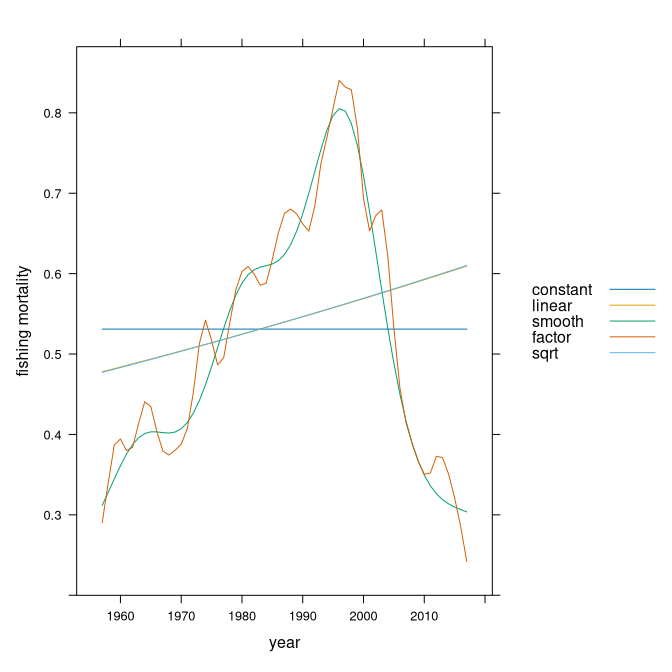
\includegraphics[width=.9\linewidth]{figure/fund_forms-1} 

}

\caption[Example of fundamental R formulas]{Example of fundamental R formulas}\label{fig:fund_forms}
\end{figure}

\end{knitrout}

The models above and their combinations can be used to model both 'age' and 'year'. The corresponding fits for age are:

\begin{knitrout}
\definecolor{shadecolor}{rgb}{0.949, 0.949, 0.949}\color{fgcolor}\begin{kframe}
\begin{alltt}
\hlcom{# models}
\hldef{m1} \hlkwb{<-} \hlopt{~}\hlnum{1}
\hldef{m2} \hlkwb{<-} \hlopt{~}\hldef{age}
\hldef{m3} \hlkwb{<-} \hlopt{~}\hlkwd{s}\hldef{(age,} \hlkwc{k} \hldef{=} \hlnum{3}\hldef{)}
\hldef{m4} \hlkwb{<-} \hlopt{~}\hlkwd{factor}\hldef{(age)}
\hldef{m5} \hlkwb{<-} \hlopt{~}\hlkwd{sqrt}\hldef{(age)}

\hlcom{# fits}
\hldef{fit1} \hlkwb{<-} \hlkwd{sca}\hldef{(ple4, ple4.indices,} \hlkwc{fmodel} \hldef{= m1,} \hlkwc{fit} \hldef{=} \hlsng{"MP"}\hldef{)}
\hldef{fit2} \hlkwb{<-} \hlkwd{sca}\hldef{(ple4, ple4.indices,} \hlkwc{fmodel} \hldef{= m2,} \hlkwc{fit} \hldef{=} \hlsng{"MP"}\hldef{)}
\hldef{fit3} \hlkwb{<-} \hlkwd{sca}\hldef{(ple4, ple4.indices,} \hlkwc{fmodel} \hldef{= m3,} \hlkwc{fit} \hldef{=} \hlsng{"MP"}\hldef{)}
\hldef{fit4} \hlkwb{<-} \hlkwd{sca}\hldef{(ple4, ple4.indices,} \hlkwc{fmodel} \hldef{= m4,} \hlkwc{fit} \hldef{=} \hlsng{"MP"}\hldef{)}
\hldef{fit5} \hlkwb{<-} \hlkwd{sca}\hldef{(ple4, ple4.indices,} \hlkwc{fmodel} \hldef{= m5,} \hlkwc{fit} \hldef{=} \hlsng{"MP"}\hldef{)}

\hlcom{# plot}
\hldef{lst} \hlkwb{<-} \hlkwd{FLStocks}\hldef{(}\hlkwc{constant} \hldef{= ple4} \hlopt{+} \hldef{fit1,} \hlkwc{linear} \hldef{= ple4} \hlopt{+} \hldef{fit2,} \hlkwc{smooth} \hldef{= ple4} \hlopt{+} \hldef{fit3,}
    \hlkwc{factor} \hldef{= ple4} \hlopt{+} \hldef{fit4,} \hlkwc{sqrt} \hldef{= ple4} \hlopt{+} \hldef{fit5)}
\hldef{lst} \hlkwb{<-} \hlkwd{lapply}\hldef{(lst,} \hlkwa{function}\hldef{(}\hlkwc{x}\hldef{)} \hlkwd{harvest}\hldef{(x)[,} \hlsng{"2000"}\hldef{])}
\hlkwd{xyplot}\hldef{(data} \hlopt{~} \hldef{age,} \hlkwc{groups} \hldef{= qname, lst,} \hlkwc{auto.key} \hldef{= lgnd,} \hlkwc{type} \hldef{=} \hlsng{"l"}\hldef{,} \hlkwc{ylab} \hldef{=} \hlsng{"fishing mortality in 2000"}\hldef{)}
\end{alltt}
\end{kframe}\begin{figure}[H]

{\centering 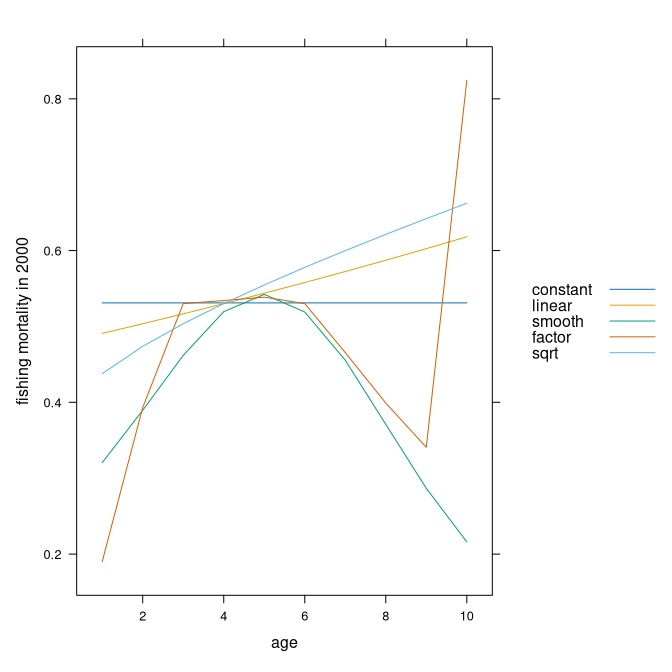
\includegraphics[width=.9\linewidth]{figure/fund_forms_age-1} 

}

\caption[Example of fundamental R formulas]{Example of fundamental R formulas}\label{fig:fund_forms_age}
\end{figure}

\end{knitrout}

\subsection{The major effects available for modelling}

Although the building blocks for formulas are 'age' and 'year', in fact there are three effects that can be modelled for each submodel: 'age', 'year' and 'cohort'. As examples note the following models for fishing mortality.

\begin{knitrout}
\definecolor{shadecolor}{rgb}{0.949, 0.949, 0.949}\color{fgcolor}\begin{kframe}
\begin{alltt}
\hlcom{# the age effect}
\hldef{ageeffect} \hlkwb{<-} \hlopt{~}\hlkwd{factor}\hldef{(age)}

\hlcom{# the year effect}
\hldef{yeareffect} \hlkwb{<-} \hlopt{~}\hlkwd{factor}\hldef{(year)}

\hlcom{# the cohort}
\hldef{cohorteffect} \hlkwb{<-} \hlopt{~}\hlkwd{factor}\hldef{(year} \hlopt{-} \hldef{age)}

\hlcom{# the fits}
\hldef{fit1} \hlkwb{<-} \hlkwd{sca}\hldef{(ple4, ple4.indices,} \hlkwc{fmodel} \hldef{= yeareffect)}
\hldef{fit2} \hlkwb{<-} \hlkwd{sca}\hldef{(ple4, ple4.indices,} \hlkwc{fmodel} \hldef{= ageeffect)}
\hldef{fit3} \hlkwb{<-} \hlkwd{sca}\hldef{(ple4, ple4.indices,} \hlkwc{fmodel} \hldef{= cohorteffect)}
\end{alltt}
\end{kframe}
\end{knitrout}

and the graphical representation of the three models in Figures~\ref{fig:majeffy} to \ref{fig:majeffc}.

\begin{knitrout}
\definecolor{shadecolor}{rgb}{0.949, 0.949, 0.949}\color{fgcolor}\begin{kframe}
\begin{alltt}
\hlkwd{wireframe}\hldef{(}\hlkwd{harvest}\hldef{(fit1),} \hlkwc{main} \hldef{=} \hlsng{"year effect"}\hldef{)}
\end{alltt}
\end{kframe}\begin{figure}[H]

{\centering 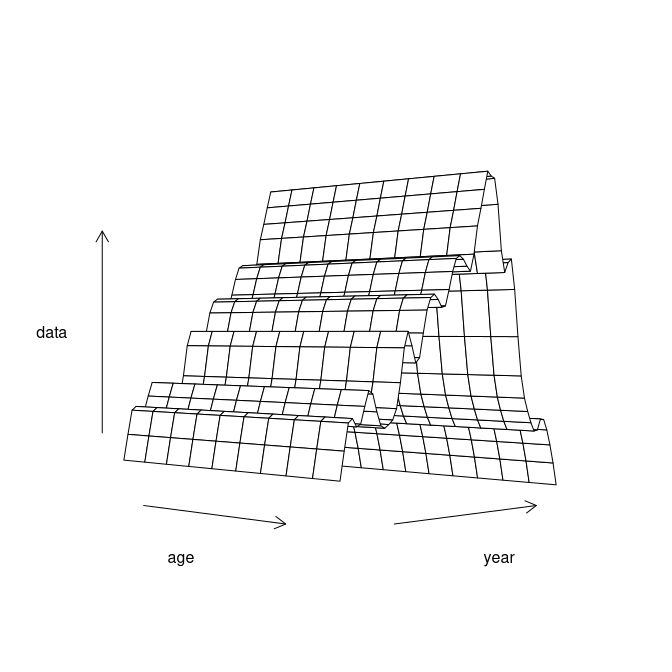
\includegraphics[width=.9\linewidth]{figure/majeffy-1} 

}

\caption[Major effects]{Major effects: the year effect (~ factor(year))}\label{fig:majeffy}
\end{figure}

\end{knitrout}

\begin{knitrout}
\definecolor{shadecolor}{rgb}{0.949, 0.949, 0.949}\color{fgcolor}\begin{kframe}
\begin{alltt}
\hlkwd{wireframe}\hldef{(}\hlkwd{harvest}\hldef{(fit2),} \hlkwc{main} \hldef{=} \hlsng{"age effect"}\hldef{)}
\end{alltt}
\end{kframe}\begin{figure}[H]

{\centering 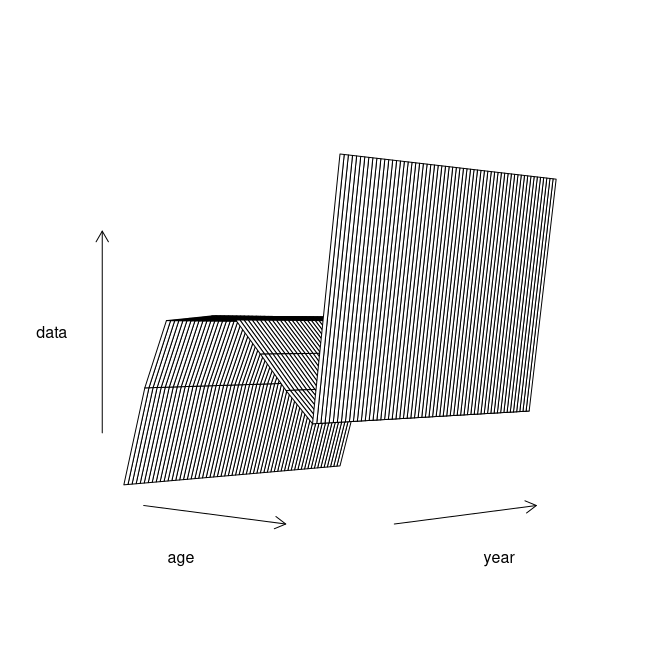
\includegraphics[width=.9\linewidth]{figure/majeffa-1} 

}

\caption[Major effects]{Major effects: the age effect (~ factor(age))}\label{fig:majeffa}
\end{figure}

\end{knitrout}

\begin{knitrout}
\definecolor{shadecolor}{rgb}{0.949, 0.949, 0.949}\color{fgcolor}\begin{kframe}
\begin{alltt}
\hlkwd{wireframe}\hldef{(}\hlkwd{harvest}\hldef{(fit3),} \hlkwc{main} \hldef{=} \hlsng{"cohort effect"}\hldef{)}
\end{alltt}
\end{kframe}\begin{figure}[H]

{\centering 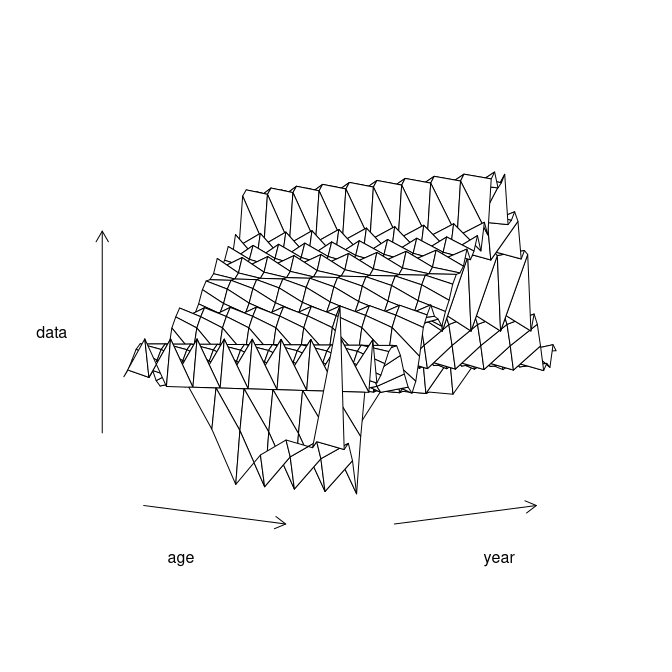
\includegraphics[width=.9\linewidth]{figure/majeffc-1} 

}

\caption[Major effects]{Major effects: the cohort effect (~ factor(year-age))}\label{fig:majeffc}
\end{figure}

\end{knitrout}

\subsection{The submodel class and methods}

%====================================================================
% COLIN TO CHECK THE SECTION
%====================================================================
%
% Although the specification of each submodel is done through a R formula, internally the \aFa sca fit creates an object (of class 'submodel') which stores more information and allows a wide number of methods to be applied. The most important cases are prediction and simulation methods.
%
% The submodel class is a S4 class with the following slots:
%
% <<>>=
% showClass("submodel")
% @
%
% Objects of class 'submodel' are created in the fitting process using the formulas set by the user (or defaults if missing) and information from the fit. 
%
% For example begining with a simple \aFa fit:
%
% <<>>=
% # fit a model with indices "IBTS_Q1" and "IBTS_Q3"
% fit0 <- sca(ple4, ple4.indices[c("IBTS_Q1", "IBTS_Q3")],
%             fmodel = ~ s(age, k = 5),
%             qmodel = list( ~ s(age, k = 4), ~ s(age, k = 4)),
%             srmodel = ~ 1,
%             n1model = ~ s(age, k = 5),
%             vmodel = list( ~ 1, ~ 1, ~ 1),
%             verbose = FALSE)
% fit0
% @
%
% Within the sca fit object there's a collection of submodels for each component of the \aFa stock assessment model (fishing mortality, survey catchability, stock recruitment relationship, initial population and the observation variance for catch numbers and survey indices). For readability the following example will use the fishing mortality submodel although the methods and models described can be applied to each of the 5 submodels.
%
% The submodel can be extracted using:
%
% <<>>=
% fmod <- fmodel(fit0)
% @
%
% inside this object is a formula, the coeficients estimated by the model and their covariance matrix.
%
% <<sim_pred_fmodel_coef, results = 'hide', eval=FALSE>>=
% coef(fmod)
% vcov(fmod)
% @
%
% it is also possible to get the data behind the fit and the design matrix required to get the fitted values
%
% <<results = 'hide', eval=FALSE>>=
% as.data.frame(fmod)
% getX(fmod)
% @
%
% this makes it possble to check the fit manually like this (note that the data is centered in the model, which is addressed by adding the centering after the prediction is made, see code below):
%
% <<eval=FALSE>>= 
% dat <- as.data.frame(fmod)
% X <- getX(fmod)
% b <- coef(fmod)
% dat$fit <- exp(c(X %*% b))# + dat$data.centering)
%
% plot(fit ~ age, type = "l", data = dat[dat$year == 2016,],
%      ylab = "Estimated fishing mortality at age",
%      ylim = c(0, max(dat$fit)), las = 1)
% @
%
% or simulate from the fit by resampling based on the variance matrix of the coefficients, which is done by simulating many coefficients (here called `bsim`).
%
% <<eval=FALSE>>=
% # get the variance matrix of the coefficients and simulate
% Sigma <- vcov(fmod)[,,1]
% bsim <- mvrnorm(999, b, Sigma)
%
% fit_sim <- exp(X %*% bsim)
% dat$ci_lower <- apply(fit_sim, 1, quantile, p = 0.025)
% dat$ci_upper <- apply(fit_sim, 1, quantile, p = 0.975)
%
% plot(fit ~ age, type = "l", data = dat[dat$year == 2016,],
%      ylab = "Estimated fishing mortality at age",
%      ylim = c(0, max(dat$ci_upper)), las = 1)
% lines(ci_lower ~ age, data = dat[dat$year == 2016,], lty = 2)
% lines(ci_upper ~ age, data = dat[dat$year == 2016,], lty = 2)
% @
%
% The above code is to show how it is possible to use an FLa4a submodel to predict and simulate, and not intended to be used by the user.  The recomended way to predict from a submodel and make simulations is to use the `genFLQuant` function (and for finer control, there is also a `simulate` function).  The above example can be done using FLa4a functions as follows:
%
% <<eval=FALSE>>=
% fmod_fit <- genFLQuant(fmod)
% dat <- as.data.frame(fmod_fit)
%
% plot(data ~ age, type = "l", data = dat[dat$year == 2016,],
%      ylab = "Estimated fishing mortality at age",
%      ylim = c(0, max(dat$data)), las = 1)
% @
%
% or using the `ggplotFL` package:
%
% <<eval=FALSE>>=
% fmod_fit <- genFLQuant(fmod)
%
% ggplot(data = fmod_fit[,"2016"], aes(x = age, y = data)) + 
%   geom_point() + geom_line() + 
%   ylab("Estimated fishing mortality at age") +
%   ylim(0, max(fmod_fit))
% @
%
% and the simulations and confidence intervals are easily computed:
%
% <<eval=FALSE>>=
% # simulate 999 
% fmod_fit_sim <- genFLQuant(fmod, nsim = 999)
%
% # reduce to quantiles
% fmod_fit_sim <- quantile(fmod_fit_sim[,"2016"], c(0.025, 0.50, 0.975))
% @
%
% plotting can be done by converting to a data.frame, reshaping and using standard `ggplot2` functionality
%
% <<eval=FALSE>>=
% dat <- 
%   reshape(
%     as.data.frame(fmod_fit_sim, drop=TRUE), 
%     timevar = "iter", idvar = "age", direction = "wide"  
%   )
%
% ggplot(data=dat, aes(x = age, y = `data.50%`)) +
%   geom_ribbon(aes(ymin = `data.2.5%`, ymax = `data.97.5%`), 
%               fill="red", alpha = .15) +
%   geom_point() + geom_line() + 
%   ylab("Estimated fishing mortality at age") +
%   ylim(0, max(fmod_fit_sim))
% @
%
\section{The statistical catch-at-age stock assessment framework}\label{sec:sca}

The \aFa stock assessment framework is implemented in \R through the method \code{sca()}. The method call requires as a minimum a FLStock object and a FLIndices object, in which case the default submodels will be set by the method.

%Having described building blocks, basic formulations and effects available to build a submodel's model, it's important to look into specific formulations and relate them to commonly known representations. Note that although a large number of formulations are available for each submodel, the user must carefuly decide on the full stock assessment model being build and avoid over-paramerizing. Over-parametrization may lead to non-convergence, but may also end up not being very useful for prediction/forecasting, which is one of the main objectives of stock assessment.

\begin{knitrout}
\definecolor{shadecolor}{rgb}{0.949, 0.949, 0.949}\color{fgcolor}\begin{kframe}
\begin{alltt}
\hlkwd{data}\hldef{(ple4)}
\hlkwd{data}\hldef{(ple4.indices)}
\hldef{fit} \hlkwb{<-} \hlkwd{sca}\hldef{(ple4, ple4.indices)}
\hldef{stk} \hlkwb{<-} \hldef{ple4} \hlopt{+} \hldef{fit}
\hlkwd{plot}\hldef{(stk)}
\end{alltt}
\end{kframe}

{\centering 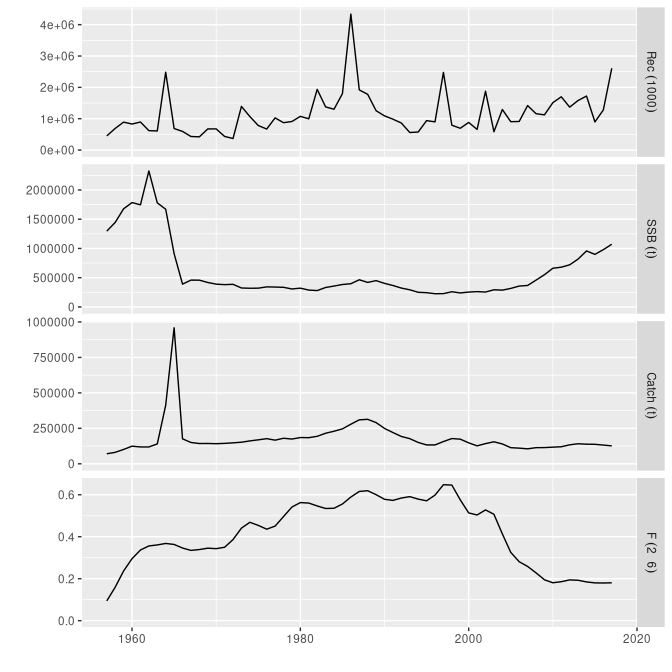
\includegraphics[width=.9\linewidth]{figure/unnamed-chunk-4-1} 

}


\end{knitrout}

By calling the fitted object the default submodel formulas are printed in the console:

\begin{knitrout}
\definecolor{shadecolor}{rgb}{0.949, 0.949, 0.949}\color{fgcolor}\begin{kframe}
\begin{alltt}
\hldef{fit}
\end{alltt}
\begin{verbatim}
## a4a model fit for: PLE 
## 
## Call:
## .local(stock = stock, indices = indices)
## 
## Time used:
##  Pre-processing     Running a4a Post-processing           Total 
##       0.8384738      13.7062440       0.1650543      14.7097721 
## 
## Submodels:
## 	 fmodel: ~te(age, year, k = c(6, 30), bs = "tp") + s(age, k = 6)
## 	srmodel: ~factor(year)
## 	n1model: ~s(age, k = 3)
## 	 qmodel:
## 	   BTS-Isis-early:                  ~s(age, k = 6)
## 	   BTS-Combined (ISIS and TRIDENS): ~s(age, k = 6)
## 	   SNS:                             ~s(age, k = 5)
## 	   BTS-Combined (all):              ~s(age, k = 6)
## 	   IBTS_Q3:                         ~s(age, k = 6)
## 	   IBTS_Q1:                         ~s(age, k = 5)
## 	 vmodel:
## 	   catch:                           ~s(age, k = 3)
## 	   BTS-Isis-early:                  ~1
## 	   BTS-Combined (ISIS and TRIDENS): ~1
## 	   SNS:                             ~1
## 	   BTS-Combined (all):              ~1
## 	   IBTS_Q3:                         ~1
## 	   IBTS_Q1:                         ~1
\end{verbatim}
\end{kframe}
\end{knitrout}

To set specific submodels the user has to write the relevant R formula and include it in the call. The arguments for each submodel are self-explanatory: fishing mortality is 'fmodel', indices' catchability is 'qmodel', stock-recruitment is 'srmodel', observation variance is 'vmodel' and for initial year's abundance is 'n1model'. The following model comes closer to the official stock assessment of North Sea plaice, as such we'll name it $0$ and keep it for future comparisons:


For future referencing we'll start with a base fit to be used for future comparisons, named fit 0.




\begin{knitrout}
\definecolor{shadecolor}{rgb}{0.949, 0.949, 0.949}\color{fgcolor}\begin{kframe}
\begin{alltt}
\hldef{fmod0} \hlkwb{<-} \hlopt{~}\hlkwd{s}\hldef{(age,} \hlkwc{k} \hldef{=} \hlnum{6}\hldef{)} \hlopt{+} \hlkwd{s}\hldef{(year,} \hlkwc{k} \hldef{=} \hlnum{10}\hldef{)} \hlopt{+} \hlkwd{te}\hldef{(age, year,} \hlkwc{k} \hldef{=} \hlkwd{c}\hldef{(}\hlnum{3}\hldef{,} \hlnum{8}\hldef{))}
\hldef{qmod0} \hlkwb{<-} \hlkwd{list}\hldef{(}\hlopt{~}\hlkwd{s}\hldef{(age,} \hlkwc{k} \hldef{=} \hlnum{4}\hldef{),} \hlopt{~}\hlkwd{s}\hldef{(age,} \hlkwc{k} \hldef{=} \hlnum{3}\hldef{),} \hlopt{~}\hlkwd{s}\hldef{(age,} \hlkwc{k} \hldef{=} \hlnum{3}\hldef{)} \hlopt{+} \hldef{year,} \hlopt{~}\hlkwd{s}\hldef{(age,} \hlkwc{k} \hldef{=} \hlnum{3}\hldef{),}
    \hlopt{~}\hlkwd{s}\hldef{(age,} \hlkwc{k} \hldef{=} \hlnum{4}\hldef{),} \hlopt{~}\hlkwd{s}\hldef{(age,} \hlkwc{k} \hldef{=} \hlnum{6}\hldef{))}
\hldef{srmod0} \hlkwb{<-} \hlopt{~}\hlkwd{s}\hldef{(year,} \hlkwc{k} \hldef{=} \hlnum{20}\hldef{)}
\hldef{vmod0} \hlkwb{<-} \hlkwd{list}\hldef{(}\hlopt{~}\hlkwd{s}\hldef{(age,} \hlkwc{k} \hldef{=} \hlnum{4}\hldef{),} \hlopt{~}\hlnum{1}\hldef{,} \hlopt{~}\hlnum{1}\hldef{,} \hlopt{~}\hlnum{1}\hldef{,} \hlopt{~}\hlnum{1}\hldef{,} \hlopt{~}\hlnum{1}\hldef{,} \hlopt{~}\hlnum{1}\hldef{,} \hlopt{~}\hlnum{1}\hldef{)}
\hldef{n1mod0} \hlkwb{<-} \hlopt{~}\hlkwd{s}\hldef{(age,} \hlkwc{k} \hldef{=} \hlnum{3}\hldef{)}
\hldef{fit0} \hlkwb{<-} \hlkwd{sca}\hldef{(ple4, ple4.indices,} \hlkwc{fmodel} \hldef{= fmod0,} \hlkwc{qmodel} \hldef{= qmod0,} \hlkwc{srmodel} \hldef{= srmod0,}
    \hlkwc{n1model} \hldef{= n1mod0,} \hlkwc{vmodel} \hldef{= vmod0)}
\hldef{stk0} \hlkwb{<-} \hldef{ple4} \hlopt{+} \hldef{fit0}
\hlkwd{plot}\hldef{(stk0)}
\end{alltt}
\end{kframe}

{\centering 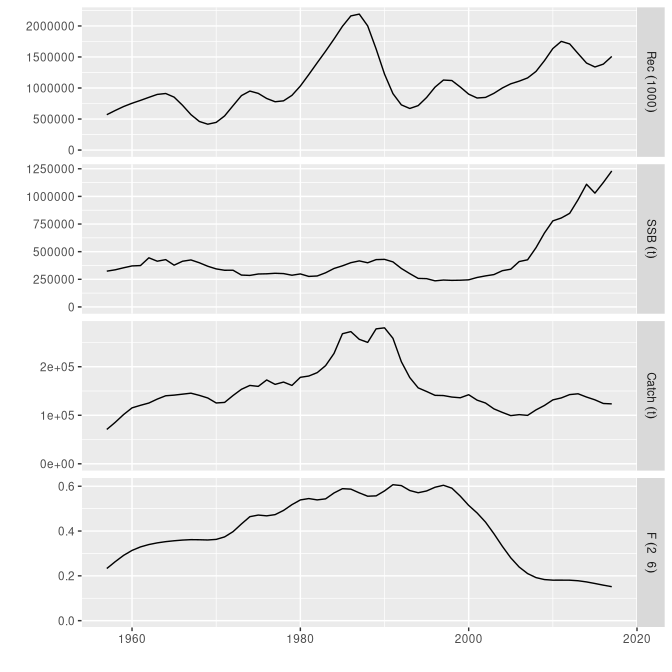
\includegraphics[width=.9\linewidth]{figure/unnamed-chunk-6-1} 

}


\end{knitrout}

As before by calling the fitted object submodels' formulas are printed in the console:

\begin{knitrout}
\definecolor{shadecolor}{rgb}{0.949, 0.949, 0.949}\color{fgcolor}\begin{kframe}
\begin{alltt}
\hldef{fit}
\end{alltt}
\begin{verbatim}
## a4a model fit for: PLE 
## 
## Call:
## .local(stock = stock, indices = indices)
## 
## Time used:
##  Pre-processing     Running a4a Post-processing           Total 
##       0.8384738      13.7062440       0.1650543      14.7097721 
## 
## Submodels:
## 	 fmodel: ~te(age, year, k = c(6, 30), bs = "tp") + s(age, k = 6)
## 	srmodel: ~factor(year)
## 	n1model: ~s(age, k = 3)
## 	 qmodel:
## 	   BTS-Isis-early:                  ~s(age, k = 6)
## 	   BTS-Combined (ISIS and TRIDENS): ~s(age, k = 6)
## 	   SNS:                             ~s(age, k = 5)
## 	   BTS-Combined (all):              ~s(age, k = 6)
## 	   IBTS_Q3:                         ~s(age, k = 6)
## 	   IBTS_Q1:                         ~s(age, k = 5)
## 	 vmodel:
## 	   catch:                           ~s(age, k = 3)
## 	   BTS-Isis-early:                  ~1
## 	   BTS-Combined (ISIS and TRIDENS): ~1
## 	   SNS:                             ~1
## 	   BTS-Combined (all):              ~1
## 	   IBTS_Q3:                         ~1
## 	   IBTS_Q1:                         ~1
\end{verbatim}
\end{kframe}
\end{knitrout}

The method \code{sca} has other arguments which may be set by the user:

\begin{description}
	\item [covar:] a \code{FLQuant} with covariates; 
	\item [wkdir:] a folder (character) where the \ADMB files will be saved for posterior inspection by the user;
	\item [verbose:] be more verbose (logical);
	\item [fit:] type of fit (character), 
	\begin{itemize}
	  \item 'MP' runs the minimizer without trying to invert the hessian and as such doesn't return the covariance matrix of the parameters, normally used inside \MSE loops where parameter variance may not be relevant; 
	  \item 'assessment' runs minimizer and inverts hessian, returns the covariance matrix of the estimated parameters and the convergence criteria set in \ADMB; 
	  \item 'MCMC' runs \ADMB's MCMC fit
	\end{itemize} 
	\item [center:] shall observations be centered before fitting (logical);
	\item [mcmc:] \ADMB's MCMC arguments (character vector), must be paired with \code{fit="MCMC"}. 
\end{description}

There are a set of methods for \aFa fit objects which help manipulating \code{sca()} results, namely:

\begin{description}
	\item [+:] update the stock object with the fitted fishing mortalities, population abundance and catch in numbers at age; 
\end{description}


\subsection{Fishing mortality submodel ($F_{ay}$)}



We will now take a look at some examples for $F$ models and the forms that we can get.

% A non-separable model, where we consider age and year to interact can be modeled using a smooth interaction term in the F model using a tensor product of cubic splines with the `te` method (`r fign('te1')`), again borrowed from [mgcv](http://cran.r-project.org/web/packages/mgcv/index.html).
%
% <<>>=
% fmod <- ~ te(age, year, k = c(4,20))
% fit <- sca(ple4, ple4.indices[1], fmod)
% @
%
% <<te1, fig.cap="Fishing mortality smoothed non-separable model">>=
% wireframe(harvest(fit), zlab="F")
% @
%
% In the last examples the fishing mortalities (Fs') are linked across age and time.  What if we want to free up a specific age class because in the residuals we see a consistent pattern.  This can happen, for example, if the spatial distribution of juveniles is disconnected to the distribution of adults.  The fishery focuses on the adult fish, and therefore the the F on young fish is a function of the distribution of the juveniles and could deserve a specific model. This can be achieved by adding a component for the year effect on age 1 (`r fign('age1')`).
%
% <<>>=
% fmod <- ~ te(age, year, k = c(4,20)) + s(year, k = 5, by = as.numeric(age==1))
% fit <- sca(ple4, ple4.indices[1], fmod)
% @
%
% <<age1, fig.cap="Fishing mortality age-year interaction model with extra age 1 smoother.">>= 
% wireframe(harvest(fit), zlab="F")
% @
%
\subsubsection{Separable model}

One of the most useful models for fishing mortality is one in which 'age' and 'year' effects are independent, that is, where the shape of the selection pattern does not change over time, but the overall level of fishing mortality do. Commonly called a 'separable model'. 

A full separable model in \aFa is written using the \code{factor} function which converts age and year effects into categorical values, forcing a different coefficient to be estimated for each level of both effects. This model has \code{age x year} number of parameters.

\begin{knitrout}
\definecolor{shadecolor}{rgb}{0.949, 0.949, 0.949}\color{fgcolor}\begin{kframe}
\begin{alltt}
\hldef{fmod1} \hlkwb{<-} \hlopt{~}\hlkwd{factor}\hldef{(age)} \hlopt{+} \hlkwd{factor}\hldef{(year)}
\hldef{fit1} \hlkwb{<-} \hlkwd{sca}\hldef{(ple4, ple4.indices,} \hlkwc{fmodel} \hldef{= fmod1,} \hlkwc{fit} \hldef{=} \hlsng{"MP"}\hldef{)}
\end{alltt}
\end{kframe}
\end{knitrout}

One can reduce the number of parameters and add dependency along both effects, although still keeping independence of each other, by using smoothers rather than \code{factor}. We'll use a (unpenalised) thin plate spline provided by package \href{http://cran.r-project.org/web/packages/mgcv/}{mgcv} method \code{s()}. We're using the North Sea Plaice data, and since it has 10 ages we will use a simple rule of thumb that the spline should have fewer than $\frac{10}{2} = 5$ degrees of freedom, and so we opt for 4 degrees of freedom. We will also do the same for year and model the change in $F$ through time as a smoother with 20 degrees of freedom.

\begin{knitrout}
\definecolor{shadecolor}{rgb}{0.949, 0.949, 0.949}\color{fgcolor}\begin{kframe}
\begin{alltt}
\hldef{fmod2} \hlkwb{<-} \hlopt{~}\hlkwd{s}\hldef{(age,} \hlkwc{k} \hldef{=} \hlnum{4}\hldef{)} \hlopt{+} \hlkwd{s}\hldef{(year,} \hlkwc{k} \hldef{=} \hlnum{20}\hldef{)}
\hldef{fit2} \hlkwb{<-} \hlkwd{sca}\hldef{(ple4, ple4.indices,} \hlkwc{fmodel} \hldef{= fmod2,} \hlkwc{fit} \hldef{=} \hlsng{"MP"}\hldef{)}
\end{alltt}
\end{kframe}
\end{knitrout}

An interesting extension of the separable model is the 'double separable' where a third factor or smoother is added for the cohort effect.

\begin{knitrout}
\definecolor{shadecolor}{rgb}{0.949, 0.949, 0.949}\color{fgcolor}\begin{kframe}
\begin{alltt}
\hldef{fmod3} \hlkwb{<-} \hlopt{~}\hlkwd{s}\hldef{(age,} \hlkwc{k} \hldef{=} \hlnum{4}\hldef{)} \hlopt{+} \hlkwd{s}\hldef{(year,} \hlkwc{k} \hldef{=} \hlnum{20}\hldef{)} \hlopt{+} \hlkwd{s}\hldef{(}\hlkwd{as.numeric}\hldef{(year} \hlopt{-} \hldef{age),} \hlkwc{k} \hldef{=} \hlnum{10}\hldef{)}
\hldef{fit3} \hlkwb{<-} \hlkwd{sca}\hldef{(ple4, ple4.indices,} \hlkwc{fmodel} \hldef{= fmod3,} \hlkwc{fit} \hldef{=} \hlsng{"MP"}\hldef{)}
\end{alltt}


{\ttfamily\noindent\bfseries\color{errorcolor}{\#\# Error in file(file, "{}r"{}): cannot open the connection}}\end{kframe}
\end{knitrout}

Figures~\ref{fig:sep00} and \ref{fig:sep01} depicts the three models selectivities for each year. Each separable model has a single selectivity that changes it's overall scale in each year, while the double separable introduces some variability over time by modeling the cohort factor.



















































































































































